% !TeX spellcheck = da_DK
\subsection{Filter}
\subsubsection{Teori og design}
Efter signalet er blevet forstærket skal det filtreres, så alle de uønskede signaler kan dæmpes. Der benyttes kun et lavpasfilter, da det ønskede signal ligger i frekvensområdet 0-10 Hz, som beskrevet i afsnit \ref{FilterAfs} på side \pageref{FilterAfs}. Filtre kan udarbejdes både i aktiv og passiv form. Hvis signalet ligger i frekvensområdet under 1 MHz anbefales det at benytte aktive filtre \cite{Carter2013}. Aktive filtre benytter operationforstærkere, kondensatorer og modstande, hvor passive filtre benytter kondensatorer, modstande og spoler \cite{Carter2013}. Der findes flere forskellige typer filtre, heriblandt Butterworth-, Tschebyschev- og Besselfilter. Butterworthfilteret giver maksimal fladhed i pasbåndet og stopbåndet. Tschebyschevfilteret giver den hurtigste overgang fra pasbåndet til stopbåndet. Besselfilteret giver en lineær faserespons, hvilket vil sige at fasen er lineær med frekvensen.\fxnote{Til os: Fasen angiver hvor godt et signals frekvensspektrum bliver gengivet}\fxnote{skal vi have et billede ind af de forskellige typer?} \cite{Carter2013} Butterworthfilteret benyttes til at filtrere signalet i dette forsøg, da der ønskes maksimal fladhed i pasbåndet og stopbåndet som nævnt i kravspecifikationerne for filtret.

Filtre kan laves i inverterende og ikke-inverterende konfigurationer. Der vælges i dette forsøg at benytte et ikke-inverterende filter, da dette har en høj indgangsimpedans. Herved forhindres loading af filtrets output. Loading defineres som effekten af, at et spændingsmålende instrument bruger strømmen i et kredsløb og kan være både ønsket og uønsket i et system. Der må eksempelvis gerne være loading, hvis det ønskes at tænde for en lampe eller en højtaler. Loading-effekten er derimod en uønsket effekt for dette projekts system, da der ønskes et lavt effektforbrug, hvilket giver en lang levetid. Loading reducerer den samlede strøm, som løber i kredsløbet, og trækker meget strøm fra batteriet. \\
Hvis der vælges en inverterende konfiguration for filtret, falder den samlede resistans, og der kræves derfor mere strøm for at opretholde outputspændingsniveauet. Eftersom den ikke-inverterende forstærker i filteret har høj inputimpedans, hvilket vil sige, at modstanden i operationsforstærkeren har en høj værdi, vil filterets output ikke blive påvirket af loading. \cite{Webster2009,Carter2013,Karni2014}

I afsnit \ref{FilterAfs} på side \ref{FilterAfs} blev karakteristikaene af lavpasfilteret bestemt. Der kræves en minimumsdæmpning af stopbåndet $(Amin)$ på 20 dB, der accepteres en maksimal variation af pasbåndet $(Amax)$ på 3 dB, knækfrekvensen $(\omega _p)$ er på 12 Hz, samt en stopbåndstærskel $( \omega _s)$ på 45 Hz. Nedenfor ses en illustration af hvad de forskellige karakteristka beskriver.

\begin{figure}[H]
\centering
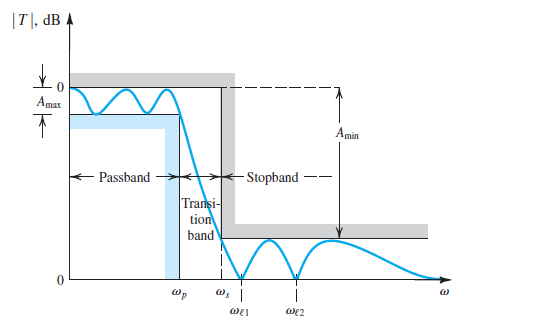
\includegraphics[scale=1]{figures/cProblemloesning/Lavpasfilter_generisk.PNG}
\caption{Figuren viser et bodeplot, hvor de fire karakteristika af et lavpasfilter er angivet.}
\label{fig:lavpasfilter_generisk}
\end{figure} 

\noindent Ud fra karakteristikaene af filteret kan filterets orden beregnes via overføringsfunktionen:
\begin{equation} \label{eq:lavpasfilter}
A(\omega_s) = 10 \text{log} \cdot \left[1 + \epsilon^2 \cdot (\frac{\omega _s}{\omega _p})^{2N}\right] 
\end{equation}

\noindent I ligning \ref{eq:lavpasfilter} er filterets orden angivet af N. Når alle de andre variable kendes, kan ordenen for filtret udregnes. I ligningen betegner $A(\omega _s)$ den minimale dæmpning der kræves af stopbåndet. $\epsilon$ er udtrykt ved ligningen:
\begin{equation}
\epsilon = \sqrt{\frac{10^{A_{max}}}{10 - 1}}
\end{equation}

Ordenen af lavpasfilteret bestemmes ved at sætte værdierne fra afsnit \ref{FilterAfs} på side \pageref{FilterAfs} ind i ligning \ref{eq:lavpasfilter}. Udregningerne vil se ud som følgende:
\begin{align}
\epsilon = \sqrt{\frac{103dB}{10 - 1}} = 0.998 \\
20\text{dB} = 10 \cdot \left[1 + 0.998^2 \frac{45\text{Hz}}{12\text{Hz}}^{2N}\right] \\
N = 1.74 \approx 2
\end{align}
\noindent Ordenen af filtret rundes op til 2, da filterets orden kun kan angives i hele tal. Hvis kravene til filteret skal overholdes, skal der altid rundes opad ved udregning af orden.

Der skal altså benyttes et 2. ordens lavpasfilter. Der findes to forskellige måder hvorpå det kan designes: Sallen-Key topologien (SKT) og Multiple Feedback toppologien (MFT). SKT-metoden er den mest anvendte og tillader separate gain indstillinger, hvorimod MFT-metoden benyttes i filter design med høj gain nøjagtighed eller høj Q værdi. For dette filter benyttes SKT. På figur \ref{fig:SallenKey} ses et 2. ordens lavpasfilter designet efter SKT. \cite{Carter2013}
\begin{figure}[H]
	\centering
	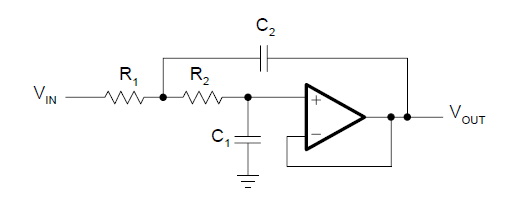
\includegraphics[scale=0.8]{figures/cProblemloesning/SallenLavpas.PNG}
	\caption{På figuren ses en illutration af et 2. ordens unity-gain Sallen-Key lavpasfilter}
	\label{fig:SallenKey}
\end{figure}

I designet af et Sallen-Key filter kræves der to modstande samt to kondensatorer. Værdierne for modstandene kan udregnes med følgende ligning:
\begin{equation} \label{eq:LavpasModstande}
R_1,2 = \frac{a_1 \cdot C_2 \pm \sqrt{A_1^2 \cdot C_2^2 - 4b_1 \cdot C_1 \cdot C_2}}{4 \pi \cdot f_c \cdot C_1 \cdot C_2}
\end{equation}

\noindent For at finde reelle værdier under kvadratroden skal følgende være opfyldt:
\begin{equation} \label{eq:kondensator}
C_2 \geq C_1 \frac{4b_1}{a_1^2}
\end{equation}
I ligning \ref{eq:LavpasModstande} står C variablene for kondensatorer, R variablene står for modstande, $a_1$ og $b_1$ er konstanter, mens $f_c$ er den valgte knækfrekvens. 

\noindent For at udregne modstandene vælges $C_1$ til at være 100nF, ud fra dette kan $C_1$ bestemmes med ligning \ref{eq:kondensator}:
\begin{equation}
C_2 \geq 100\text{nF} \frac{4\cdot 1}{1.4142^2} = C_2 \geq 200\text{nF}
\end{equation}

\noindent Ud fra ovenstående ligning vælges $C_2$ til at være 480nF, dermed kan $R_1$ og $R_2$ beregnes med ligning \ref{eq:LavpasModstande}:
\begin{equation}
R_{1,2} = \frac{1.4142 \cdot 480\text{nF} \pm \sqrt{1.4142^2 \cdot 480\text{nF}^2 - 4 \cdot 1 \cdot 100\text{nF} \cdot 480\text{nF}}}{4 \pi \cdot 12\text{Hz} \cdot 100\text{nF} \cdot 480\text{nF}} = \begin{cases} R_{1} = 16540 \Omega \\ R_{2} = 2215.53 \Omega \end{cases}
\end{equation}

\noindent Kondensatorernes samt modstandenes værdier er hermed udregnet. Disse kan nu indsættes i LT Spice, hvorefter filtret kan simuleres. 

\begin{figure}[H]
	\centering
	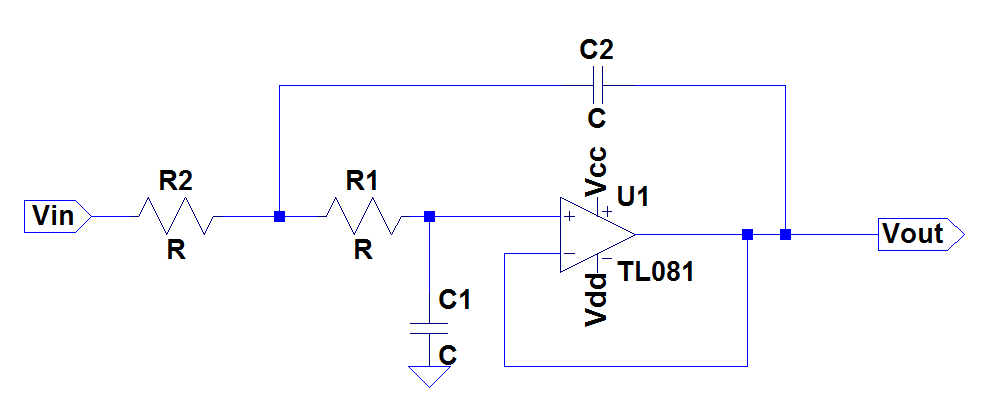
\includegraphics[scale=0.58]{figures/cProblemloesning/Lavpasfilter_teoretisk.PNG}
	\caption{På figuren ses det teoretiske kredsløb for lavpasfilteret tegnet i LT Spice.}
	\label{fig:lavpasfilter_teoretisk}
\end{figure}